\documentclass[12pt,a4paper]{ctexart}

\usepackage[a4paper,margin=2.2cm]{geometry}
\usepackage{graphicx}
\usepackage{booktabs}
\usepackage{array}
\usepackage{longtable}
\usepackage{float}
\usepackage{siunitx}
\usepackage{xcolor}
\usepackage{hyperref}
\usepackage{caption}
\usepackage{setspace}
\usepackage{enumitem}

\hypersetup{
  colorlinks=true,
  linkcolor=blue!50!black,
  urlcolor=blue!50!black,
  pdftitle={NF10 仅采样噪声条件下 FIA 与电压型 KT/C 方案详细对比报告},
  pdfauthor={Codex}
}

\captionsetup{font=small,labelfont=bf}
\setstretch{1.20}
\setlist[itemize]{nosep,leftmargin=2em}
\sisetup{
  round-mode=places,
  round-precision=4,
  group-separator={,}
}

\title{\textbf{NF10 仅采样噪声条件下}\\[4pt]\textbf{FIA 与电压型 KT/C 方案详细对比报告}}
\author{项目整理日期：2026-06-09}
\date{}

\begin{document}
\maketitle
\tableofcontents
\newpage

\section{报告目的}

本报告用于对 12bit 50M SAR ADC 在 \texttt{NOISEFACTOR=10}、仅打开采样噪声条件下的两组有效方案进行统一整理、计算和解释，并给出一份可直接引用的正式结论。

本报告只采用当前确认后的口径：

\begin{itemize}
  \item 昨天 FIA sweep 数据为正式基准，也就是当前的“方案 A”。
  \item 今天第一组电压型数据因设置较差而舍弃，不作为正式方案参与结论。
  \item 今天后面读到的电压型数据，才是正式对比用电压型 KT/C 方案。
\end{itemize}

\section{测量口径与基准定义}

\subsection{噪声设置}

\begin{itemize}
  \item 测试条件：仅打开采样噪声。
  \item \texttt{NOISEFACTOR=10}：采样噪声电压放大 10 倍，对应噪声功率放大 100 倍。
  \item corner 覆盖：\texttt{tt}、\texttt{ff}、\texttt{ss}、\texttt{sf}、\texttt{fs}。
  \item 主要观测指标：ENOB、SNR、SFDR、Power、COMPOWER。
\end{itemize}

\subsection{原本基准}

将昨天 FIA sweep 中的 \texttt{td=24.05n} 作为“原本”基准。其对应 AZ 时间仅约 \SI{0.05}{ns}，可近似视为未充分完成采样噪声消除。

该基准的平均指标为：

\begin{itemize}
  \item ENOB = \num{8.7524} bit
  \item SNR = \SI{54.3396}{dB}
  \item SFDR = \SI{66.6875}{dB}
  \item Power = \SI{294.4974}{uW}
\end{itemize}

\subsection{噪声功率百分比计算方法}

本报告中，采样噪声功率剩余百分比与消除百分比统一按 SNR 差值折算：

\begin{equation}
\Delta SNR = SNR_{\text{after}} - SNR_{\text{baseline}}
\end{equation}

\begin{equation}
\text{剩余噪声功率百分比} = 100 \times 10^{-\Delta SNR / 10}
\end{equation}

\begin{equation}
\text{噪声功率消除百分比} = 100 - \text{剩余噪声功率百分比}
\end{equation}

这里 baseline 统一取昨天 FIA 的 \texttt{td=24.05n}。

\section{昨天 FIA sweep 结果}

\subsection{三组 td 数据}

\begin{table}[H]
\centering
\caption{昨天 FIA sweep 汇总结果}
\begin{tabular}{>{\raggedright\arraybackslash}p{2.8cm}cccc}
\toprule
td / AZ & ENOB avg & SNR avg / dB & SFDR avg / dB & Power avg / uW \\
\midrule
\texttt{24.05n / 0.05ns} & 8.7524 & 54.3396 & 66.6875 & 294.4974 \\
\texttt{26n / 2ns} & 10.3399 & 63.9148 & 75.8884 & 303.6580 \\
\texttt{28n / 4ns} & 10.3484 & 63.9574 & 75.6688 & 307.8167 \\
\bottomrule
\end{tabular}
\end{table}

\subsection{相对于原本基准的采样噪声消除}

\begin{table}[H]
\centering
\caption{昨天 FIA 相对原本基准的噪声功率变化}
\begin{tabular}{>{\raggedright\arraybackslash}p{2.8cm}ccc}
\toprule
td / AZ & $\Delta SNR$ / dB & 剩余噪声功率 & 噪声功率消除 \\
\midrule
\texttt{26n / 2ns} & 9.5752 & 11.03\% & 88.97\% \\
\texttt{28n / 4ns} & 9.6178 & 10.92\% & 89.08\% \\
\bottomrule
\end{tabular}
\end{table}

从结果上看，FIA 的主要采样噪声消除已经在约 \SI{2}{ns} AZ 时间内完成。继续从 \SI{2}{ns} 延长到 \SI{4}{ns}，平均 SNR 仅再提升约 \SI{0.0426}{dB}，收益很小。

\section{正式电压型方案结果}

\subsection{方案平均结果}

正式对比用电压型方案位于 \texttt{td=28n / AZ\textasciitilde4ns}，平均结果如下：

\begin{table}[H]
\centering
\caption{正式电压型方案平均指标}
\small
\begin{tabular}{>{\centering\arraybackslash}p{2.1cm}>{\centering\arraybackslash}p{2.1cm}>{\centering\arraybackslash}p{2.3cm}>{\centering\arraybackslash}p{2.3cm}>{\centering\arraybackslash}p{2.5cm}}
\toprule
ENOB avg / bit & SNR avg / dB & SFDR avg / dB & Power avg / uW & COMPOWER avg / uW \\
\midrule
10.6807 & 66.1743 & 77.9141 & 439.8245 & 236.2862 \\
\bottomrule
\end{tabular}
\normalsize
\end{table}

\subsection{相对于原本基准的采样噪声消除}

正式电压型相对昨天 \texttt{td=24.05n} 基准：

\begin{itemize}
  \item $\Delta SNR = 66.1743 - 54.3396 = \SI{11.8347}{dB}$
  \item 剩余噪声功率 $\approx 6.55\%$
  \item 噪声功率消除 $\approx 93.45\%$
\end{itemize}

这说明正式电压型对采样噪声的压低强于 FIA。

\section{两组最终方案的直接对比}

\subsection{平均值对比}

\begin{table}[H]
\centering
\caption{FIA td=28n 与正式电压型 td=28n 的平均对比}
\begin{tabular}{lccc}
\toprule
指标 & FIA td=28n & 正式电压型 & 电压型 - FIA \\
\midrule
ENOB / bit & 10.3484 & 10.6807 & +0.3323 \\
SNR / dB & 63.9574 & 66.1743 & +2.2169 \\
SFDR / dB & 75.6688 & 77.9141 & +2.2453 \\
Power / uW & 307.8167 & 439.8245 & +132.0078 \\
COMPOWER / uW & 176.2009 & 236.2862 & +60.0853 \\
\bottomrule
\end{tabular}
\end{table}

\subsection{逐 corner SNR 对比}

\begin{table}[H]
\centering
\caption{逐 corner SNR 对比}
\begin{tabular}{lccc}
\toprule
corner & FIA / dB & 正式电压型 / dB & 电压型 - FIA / dB \\
\midrule
tt & 65.9413 & 66.1321 & +0.1908 \\
ff & 63.5149 & 68.1704 & +4.6555 \\
ss & 63.2268 & 64.0304 & +0.8036 \\
sf & 63.9569 & 65.7646 & +1.8077 \\
fs & 63.1473 & 66.7739 & +3.6266 \\
average & 63.9574 & 66.1743 & +2.2169 \\
\bottomrule
\end{tabular}
\end{table}

从逐 corner 结果看，正式电压型方案的优势主要集中在 \texttt{ff} 与 \texttt{fs}，其中 \texttt{ff} 提升最大，达到 \SI{4.6555}{dB}。在 \texttt{tt} corner 上提升较小，但整体仍然略优于 FIA。

\subsection{相对于 FIA 的额外噪声功率改善}

如果只看“正式电压型相对于 FIA td=28n 又额外改善了多少”，则：

\begin{equation}
\Delta SNR = 66.1743 - 63.9574 = \SI{2.2169}{dB}
\end{equation}

\begin{equation}
\text{相对 FIA 的剩余噪声功率} = 100 \times 10^{-2.2169/10} \approx 60.02\%
\end{equation}

这意味着正式电压型相对于 FIA td=28n，又额外压低了约 \textbf{39.98\%} 的噪声功率。

\section{图形化结果}

\begin{figure}[H]
  \centering
  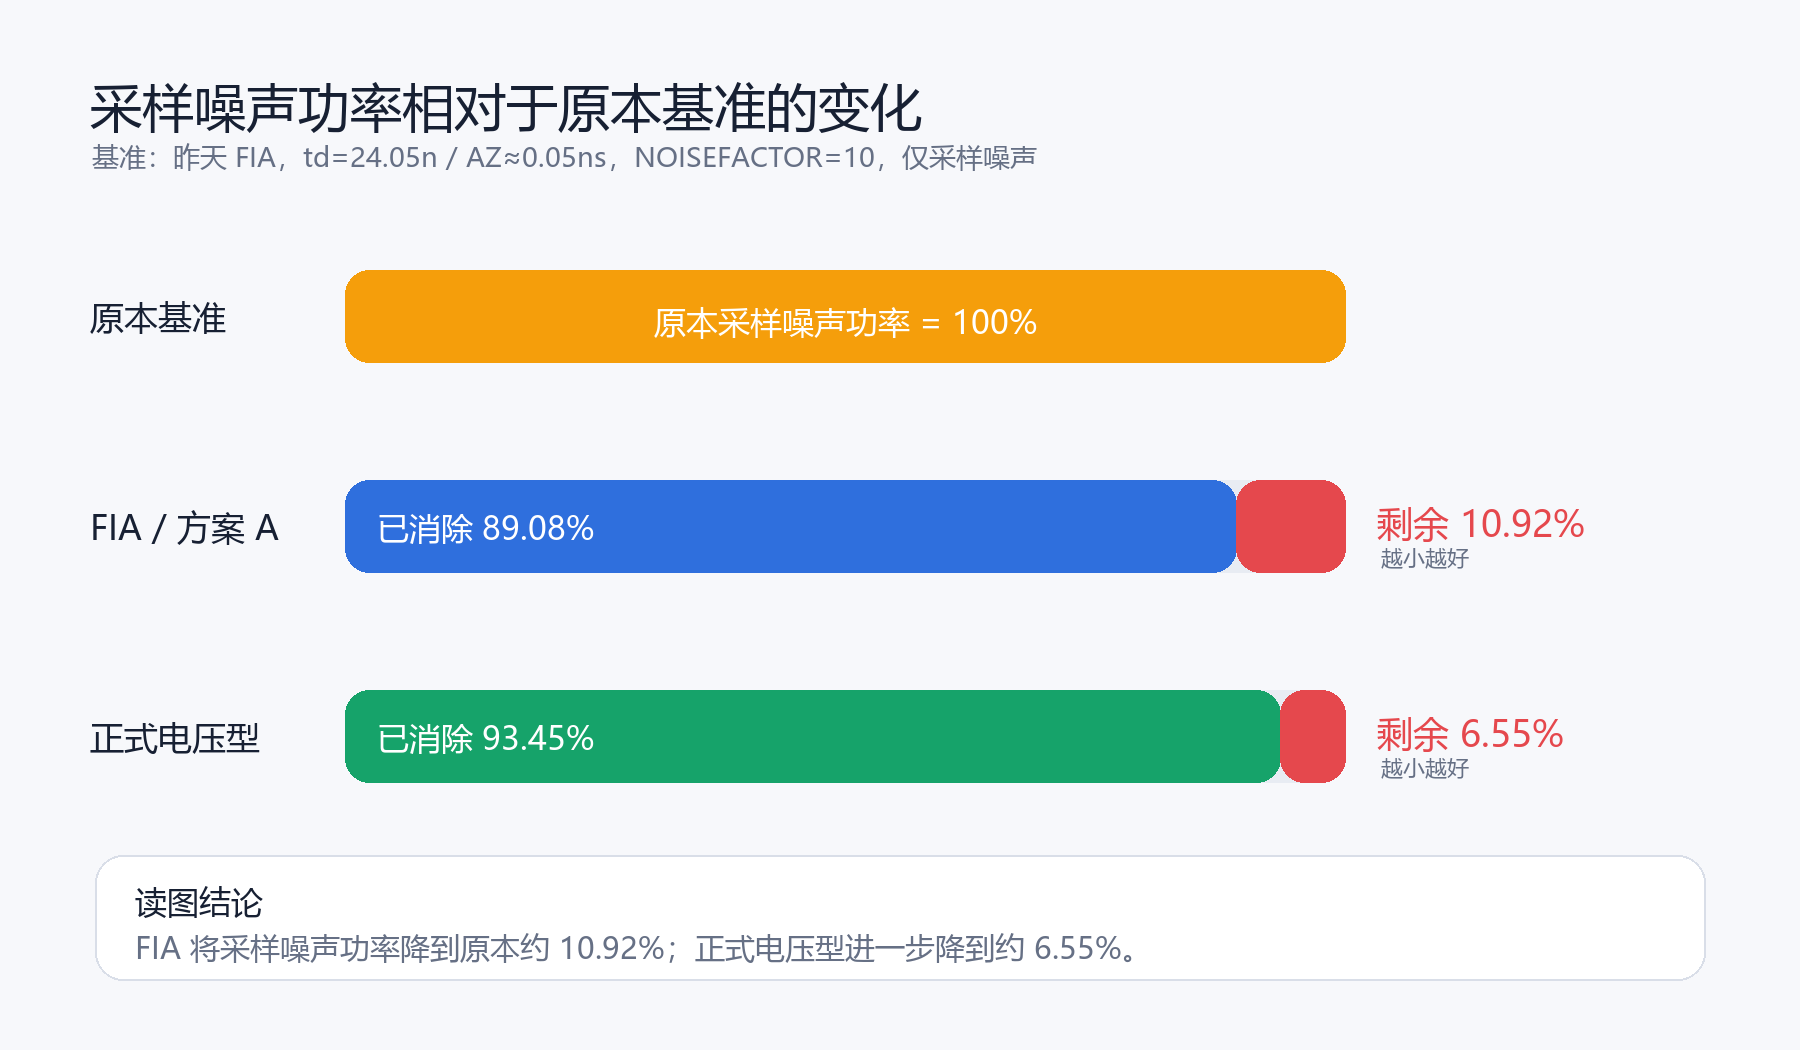
\includegraphics[width=0.95\textwidth]{../figures/2026-06-09_nf10_noise_power_reduction.png}
  \caption{相对于原本基准的采样噪声功率变化}
\end{figure}

\begin{figure}[H]
  \centering
  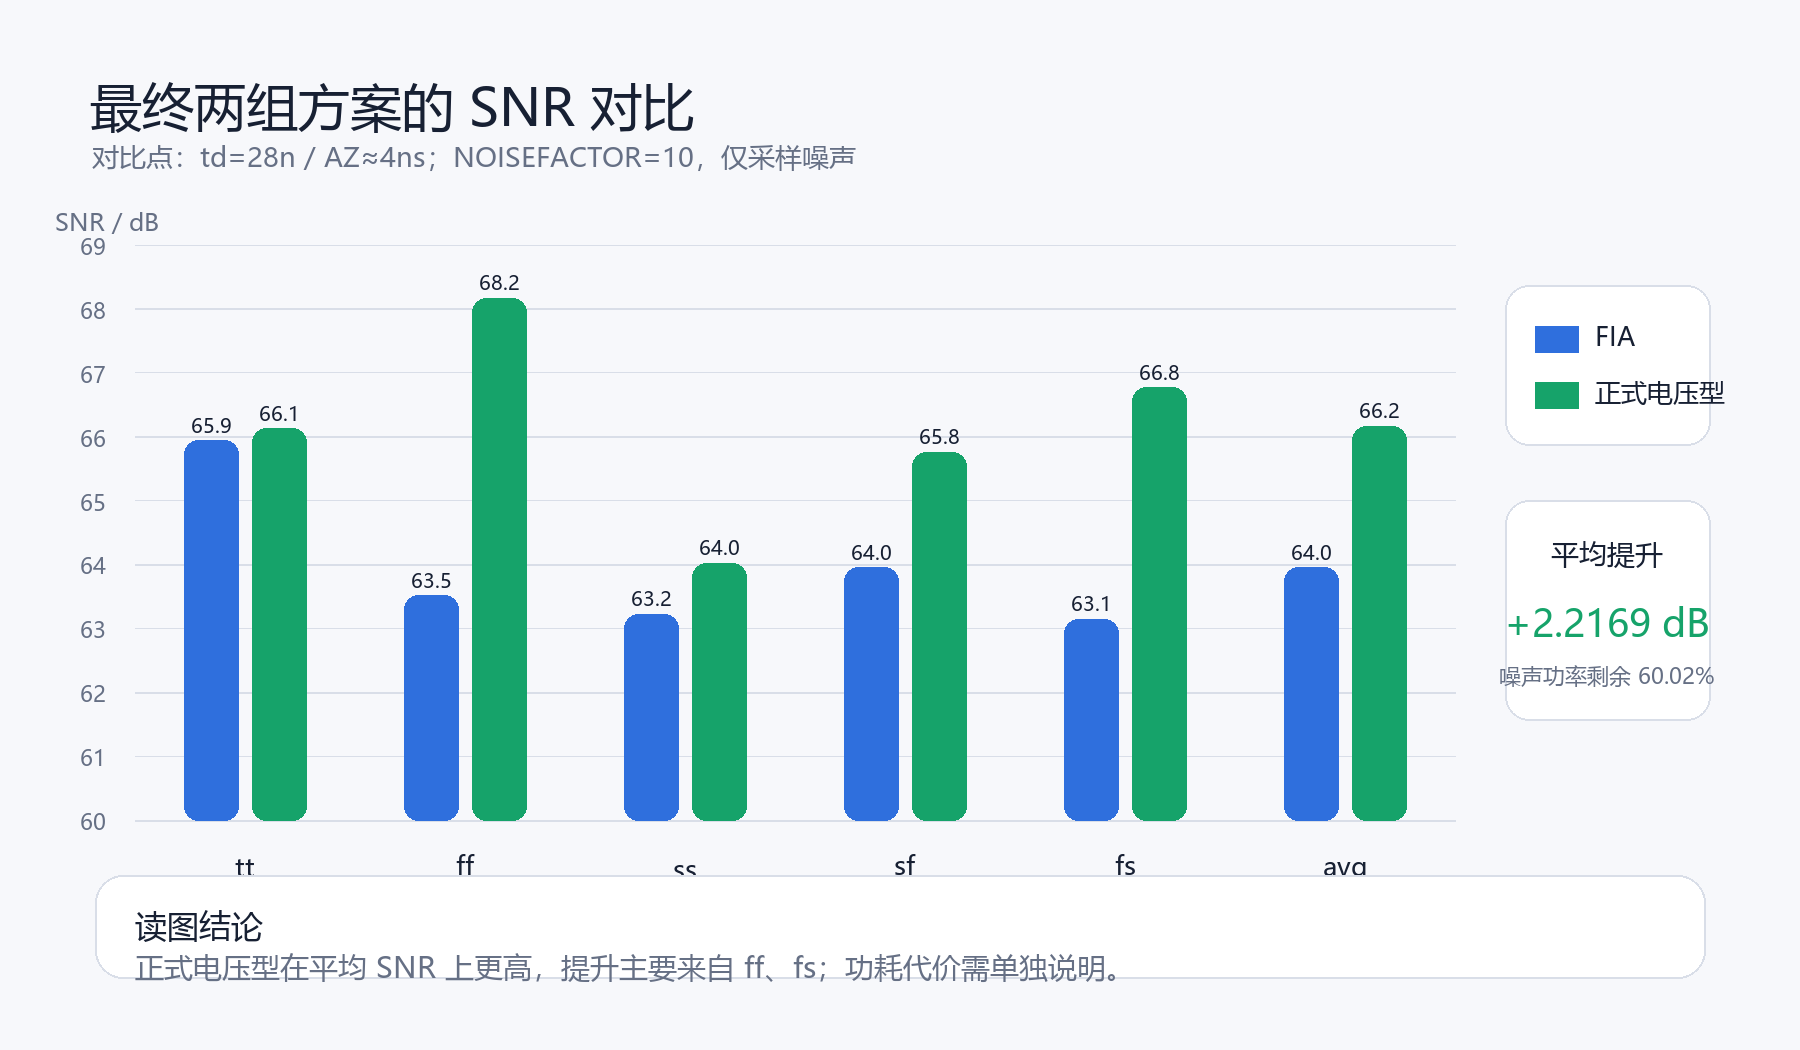
\includegraphics[width=0.95\textwidth]{../figures/2026-06-09_nf10_snr_corner_compare.png}
  \caption{FIA 与正式电压型的逐 corner SNR 对比}
\end{figure}

\section{与全噪声标称结果的关系}

全噪声标称测试结果为：

\begin{table}[H]
\centering
\caption{全噪声标称参考结果}
\begin{tabular}{>{\raggedright\arraybackslash}p{2.8cm}cccc}
\toprule
td / AZ & ENOB avg & SNR avg / dB & SFDR avg / dB & Power avg / uW \\
\midrule
\texttt{24.05n / 0.05ns} & 11.3548 & 70.3257 & 81.4859 & 361.3129 \\
\texttt{28n / 4ns} & 11.4870 & 71.2896 & 81.5728 & 374.4972 \\
\bottomrule
\end{tabular}
\end{table}

在全噪声标称下，\texttt{td=28n} 相对 \texttt{td=24.05n} 的总噪声等效功率约降低 \textbf{19.90\%}。但这个数值不能直接解释为“纯采样噪声消除百分比”，因为全噪声条件下不只有采样噪声在起作用。

\section{最终结论}

\begin{enumerate}
  \item 昨天 FIA 在 \texttt{td=28n} 时，采样噪声功率相对原本基准约剩余 \textbf{10.92\%}，即降低约 \textbf{89.08\%}。
  \item 正式电压型方案在 \texttt{td=28n} 时，采样噪声功率相对原本基准约剩余 \textbf{6.55\%}，即降低约 \textbf{93.45\%}。
  \item 正式电压型相对 FIA \texttt{td=28n} 的平均 SNR 提升为 \textbf{\SI{2.2169}{dB}}，等效于噪声功率进一步降低约 \textbf{39.98\%}。
  \item 正式电压型的优点是采样噪声压低更强、平均 SNR/ENOB/SFDR 更高；缺点是平均总功耗增加约 \textbf{\SI{132.01}{uW}}。
  \item 若后续汇报重点是“采样噪声消除能力”，正式电压型更强；若后续进入电路最终取舍，则必须同时呈现其功耗代价。
\end{enumerate}

\end{document}
